\documentclass[aspectratio=169]{beamer}
\usetheme{Madrid}
\usecolortheme{default}
\usepackage{booktabs}
\usepackage{graphicx}
\usepackage{amsmath}

\title{DQN and Double DQN for CartPole-v1}
\subtitle{A Reproducible DATA8007 Reinforcement Learning Study}
\author{Jianyu Zhang\\Student number: 3030114491}
\institute{DATA8007 Foundations of Sequential Decision-Making}
\date{2025}

\begin{document}

\begin{frame}
  \titlepage
\end{frame}

\begin{frame}{Project Question}
\begin{itemize}
  \item Can a compact PyTorch implementation reproduce DQN and Double DQN on Gymnasium CartPole-v1?
  \item Does Double DQN improve performance or stability under the same hyperparameters?
  \item How much seed sensitivity appears in a small deep RL experiment?
\end{itemize}
\end{frame}

\begin{frame}{Problem Setting}
\begin{itemize}
  \item Environment: Gymnasium CartPole-v1.
  \item Observation: four continuous state variables.
  \item Action space: two discrete actions.
  \item Maximum episode length: 500 steps.
  \item Solved threshold: average return near 475.
\end{itemize}
\end{frame}

\begin{frame}{DQN Baseline}
\begin{itemize}
  \item Q-network: MLP with hidden sizes $[128,128]$ and ReLU activations.
  \item Stabilization: experience replay and a target network.
  \item Optimization: Adam, Smooth L1 loss, batch size 64.
  \item Exploration: epsilon-greedy schedule from 1.0 to 0.05.
\end{itemize}
\[ y^{DQN}=r+\gamma(1-d)\max_{a^{\prime}}Q_{\theta^-}(s^{\prime},a^{\prime}) \]
\end{frame}

\begin{frame}{Double DQN Comparison}
\begin{itemize}
  \item Double DQN uses the online network to select the next action.
  \item The target network evaluates the selected action.
  \item This can reduce overestimation bias from the max operator.
\end{itemize}
\[ a^*=\arg\max_{a^{\prime}}Q_{\theta}(s^{\prime},a^{\prime}),\quad y^{Double}=r+\gamma(1-d)Q_{\theta^-}(s^{\prime},a^*) \]
\end{frame}

\begin{frame}{Experimental Design}
\begin{itemize}
  \item Algorithms: DQN and Double DQN.
  \item Seeds: 0, 1, and 2 for each method.
  \item Training budget: 160 episodes.
  \item Evaluation: five greedy episodes every 20 training episodes.
  \item Final checkpoint evaluation: 20 greedy episodes with evaluation seed 12345.
  \item Hardware: NVIDIA L40S GPU when CUDA is available.
\end{itemize}
\end{frame}

\begin{frame}{Training Curves}
\begin{center}
  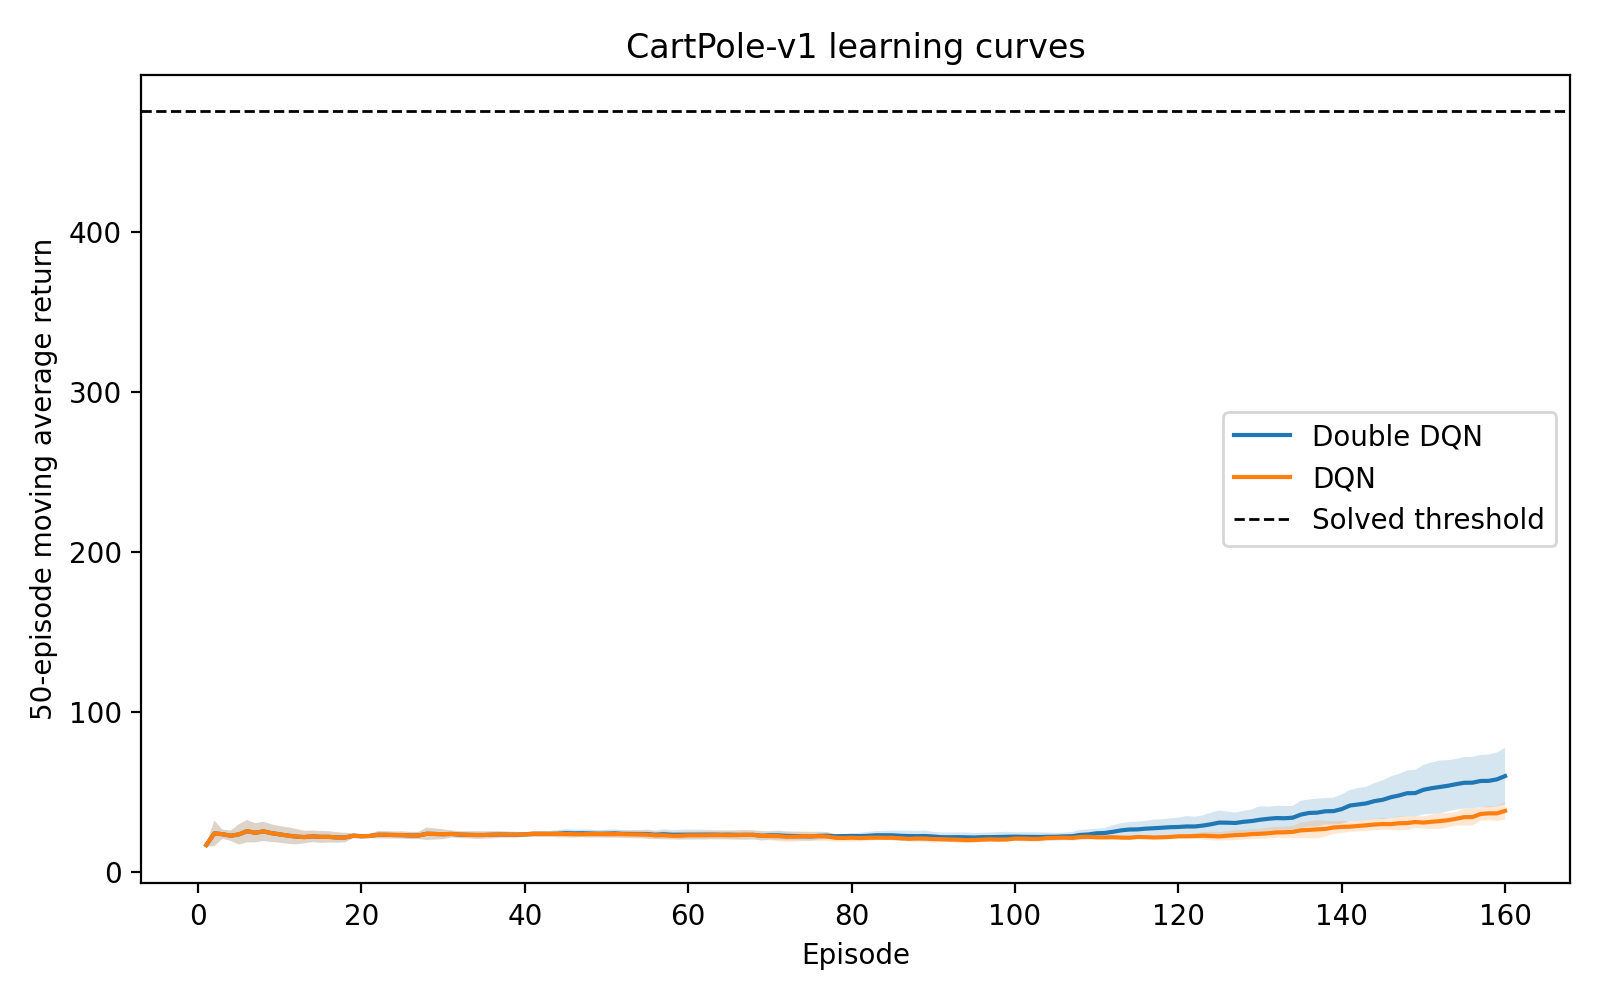
\includegraphics[width=0.88\linewidth]{../results/figures/learning_curves.png}
\end{center}
\end{frame}

\begin{frame}{Evaluation Curves}
\begin{center}
  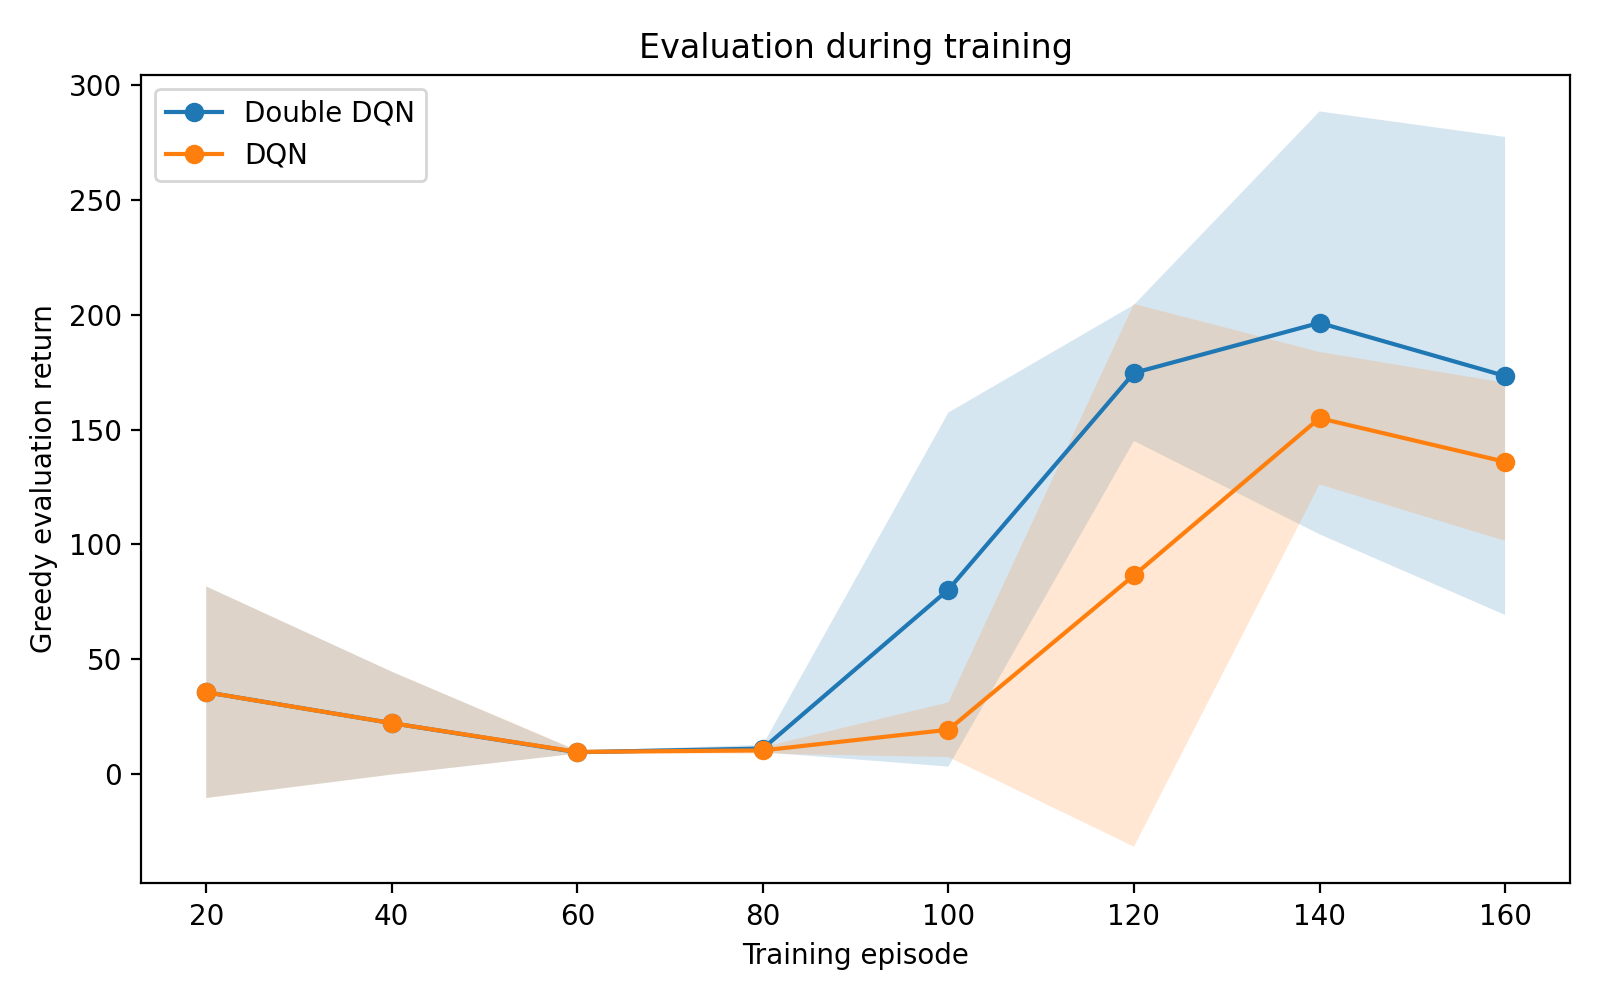
\includegraphics[width=0.88\linewidth]{../results/figures/evaluation_curves.png}
\end{center}
\end{frame}

\begin{frame}{Summary Results}
\begin{table}
\centering
\begin{tabular}{lrrr}
\toprule
Method & Final return & Final MA50 & Best eval \\
\midrule
DQN & $90.33 \pm 37.45$ & $38.37 \pm 5.46$ & $166.60 \pm 48.91$ \\
Double DQN & $160.33 \pm 57.84$ & $60.09 \pm 17.75$ & $250.93 \pm 74.79$ \\
\bottomrule
\end{tabular}
\end{table}
\begin{itemize}
  \item Double DQN achieved higher aggregate returns under the fixed budget.
  \item No run reached the CartPole solved threshold.
  \item Variance across seeds remains substantial.
\end{itemize}
\end{frame}

\begin{frame}{Reproducibility}
\begin{itemize}
  \item Configuration files define method, seeds, device, and hyperparameters.
  \item Training, evaluation, and plotting scripts save logs and figures.
  \item Results are stored in CSV, JSON, and PNG files.
  \item The repository includes the LaTeX report and this slide deck PDF.
\end{itemize}
\end{frame}

\begin{frame}{Conclusion}
\begin{itemize}
  \item The project implements a complete DQN and Double DQN workflow in PyTorch.
  \item Double DQN performed better in this controlled CartPole experiment.
  \item The conclusion is cautious because training was short and seed variance was high.
  \item Natural extensions: more seeds, longer training, prioritized replay, dueling networks, and harder environments.
\end{itemize}
\end{frame}

\end{document}
